% Options for packages loaded elsewhere
\PassOptionsToPackage{unicode}{hyperref}
\PassOptionsToPackage{hyphens}{url}
\PassOptionsToPackage{dvipsnames,svgnames,x11names}{xcolor}
%
\documentclass[
  a4paper,
]{scrreport}

\usepackage{amsmath,amssymb}
\usepackage{iftex}
\ifPDFTeX
  \usepackage[T1]{fontenc}
  \usepackage[utf8]{inputenc}
  \usepackage{textcomp} % provide euro and other symbols
\else % if luatex or xetex
  \usepackage{unicode-math}
  \defaultfontfeatures{Scale=MatchLowercase}
  \defaultfontfeatures[\rmfamily]{Ligatures=TeX,Scale=1}
\fi
\usepackage{lmodern}
\ifPDFTeX\else  
    % xetex/luatex font selection
\fi
% Use upquote if available, for straight quotes in verbatim environments
\IfFileExists{upquote.sty}{\usepackage{upquote}}{}
\IfFileExists{microtype.sty}{% use microtype if available
  \usepackage[]{microtype}
  \UseMicrotypeSet[protrusion]{basicmath} % disable protrusion for tt fonts
}{}
\makeatletter
\@ifundefined{KOMAClassName}{% if non-KOMA class
  \IfFileExists{parskip.sty}{%
    \usepackage{parskip}
  }{% else
    \setlength{\parindent}{0pt}
    \setlength{\parskip}{6pt plus 2pt minus 1pt}}
}{% if KOMA class
  \KOMAoptions{parskip=half}}
\makeatother
\usepackage{xcolor}
\setlength{\emergencystretch}{3em} % prevent overfull lines
\setcounter{secnumdepth}{-\maxdimen} % remove section numbering
% Make \paragraph and \subparagraph free-standing
\ifx\paragraph\undefined\else
  \let\oldparagraph\paragraph
  \renewcommand{\paragraph}[1]{\oldparagraph{#1}\mbox{}}
\fi
\ifx\subparagraph\undefined\else
  \let\oldsubparagraph\subparagraph
  \renewcommand{\subparagraph}[1]{\oldsubparagraph{#1}\mbox{}}
\fi


\providecommand{\tightlist}{%
  \setlength{\itemsep}{0pt}\setlength{\parskip}{0pt}}\usepackage{longtable,booktabs,array}
\usepackage{calc} % for calculating minipage widths
% Correct order of tables after \paragraph or \subparagraph
\usepackage{etoolbox}
\makeatletter
\patchcmd\longtable{\par}{\if@noskipsec\mbox{}\fi\par}{}{}
\makeatother
% Allow footnotes in longtable head/foot
\IfFileExists{footnotehyper.sty}{\usepackage{footnotehyper}}{\usepackage{footnote}}
\makesavenoteenv{longtable}
\usepackage{graphicx}
\makeatletter
\def\maxwidth{\ifdim\Gin@nat@width>\linewidth\linewidth\else\Gin@nat@width\fi}
\def\maxheight{\ifdim\Gin@nat@height>\textheight\textheight\else\Gin@nat@height\fi}
\makeatother
% Scale images if necessary, so that they will not overflow the page
% margins by default, and it is still possible to overwrite the defaults
% using explicit options in \includegraphics[width, height, ...]{}
\setkeys{Gin}{width=\maxwidth,height=\maxheight,keepaspectratio}
% Set default figure placement to htbp
\makeatletter
\def\fps@figure{htbp}
\makeatother

%\newfontfamily\Ubuntu[Mapping=tex-text]{Ubuntu}
\usepackage{pgfplots}
\usetikzlibrary{arrows.meta,arrows}
\usetikzlibrary{angles,quotes}
\pgfplotsset{grid style={dashed,mygray}}
% Colors
\definecolor{myblue}{rgb}{0.067,0.529,0.871}
\definecolor{mypurple}{rgb}{0.859,0.071,0.525}
\definecolor{myred}{rgb}{1.0, 0.13, 0.32}
\definecolor{mygreen}{rgb}{0.01, 0.75, 0.24}
\definecolor{myblack}{gray}{0.1}
\definecolor{mygray}{gray}{0.8}
\newcommand{\NN}{\mathbb{N}}
\newcommand{\ZZ}{\mathbb{Z}}
\newcommand{\QQ}{\mathbb{Q}}
\newcommand{\RR}{\mathbb{R}}
\newcommand{\CC}{\mathbb{C}}
\DeclareMathOperator{\Int}{Int}
\DeclareMathOperator{\Ext}{Ext}
\DeclareMathOperator{\Fr}{Fr}
\DeclareMathOperator{\Adh}{Adh}
\DeclareMathOperator{\Ac}{Ac}
\DeclareMathOperator{\sen}{sen}
\makeatletter
\makeatother
\makeatletter
\makeatother
\makeatletter
\@ifpackageloaded{caption}{}{\usepackage{caption}}
\AtBeginDocument{%
\ifdefined\contentsname
  \renewcommand*\contentsname{Indice de contenidos}
\else
  \newcommand\contentsname{Indice de contenidos}
\fi
\ifdefined\listfigurename
  \renewcommand*\listfigurename{Listado de Figuras}
\else
  \newcommand\listfigurename{Listado de Figuras}
\fi
\ifdefined\listtablename
  \renewcommand*\listtablename{Listado de Tablas}
\else
  \newcommand\listtablename{Listado de Tablas}
\fi
\ifdefined\figurename
  \renewcommand*\figurename{Figura}
\else
  \newcommand\figurename{Figura}
\fi
\ifdefined\tablename
  \renewcommand*\tablename{Tabla}
\else
  \newcommand\tablename{Tabla}
\fi
}
\@ifpackageloaded{float}{}{\usepackage{float}}
\floatstyle{ruled}
\@ifundefined{c@chapter}{\newfloat{codelisting}{h}{lop}}{\newfloat{codelisting}{h}{lop}[chapter]}
\floatname{codelisting}{Listado}
\newcommand*\listoflistings{\listof{codelisting}{Listado de Listados}}
\makeatother
\makeatletter
\@ifpackageloaded{caption}{}{\usepackage{caption}}
\@ifpackageloaded{subcaption}{}{\usepackage{subcaption}}
\makeatother
\makeatletter
\@ifpackageloaded{tcolorbox}{}{\usepackage[skins,breakable]{tcolorbox}}
\makeatother
\makeatletter
\@ifundefined{shadecolor}{\definecolor{shadecolor}{rgb}{.97, .97, .97}}
\makeatother
\makeatletter
\makeatother
\makeatletter
\makeatother
\ifLuaTeX
\usepackage[bidi=basic]{babel}
\else
\usepackage[bidi=default]{babel}
\fi
\babelprovide[main,import]{spanish}
% get rid of language-specific shorthands (see #6817):
\let\LanguageShortHands\languageshorthands
\def\languageshorthands#1{}
\ifLuaTeX
  \usepackage{selnolig}  % disable illegal ligatures
\fi
\IfFileExists{bookmark.sty}{\usepackage{bookmark}}{\usepackage{hyperref}}
\IfFileExists{xurl.sty}{\usepackage{xurl}}{} % add URL line breaks if available
\urlstyle{same} % disable monospaced font for URLs
\hypersetup{
  pdftitle={Diagnóstico del Glaucoma},
  pdflang={es},
  colorlinks=true,
  linkcolor={blue},
  filecolor={Maroon},
  citecolor={Blue},
  urlcolor={Blue},
  pdfcreator={LaTeX via pandoc}}

\title{Diagnóstico del Glaucoma}
\author{}
\date{}

\begin{document}
\begin{titlepage}

%\AddToShipoutPicture*{\put(0,0){\includegraphics[scale=0.8]{img/background2}}} % Imagen de fondo, requiere el paquete eso-pic.
\begin{center}
\vspace*{5cm}

\Huge
{\textbf{\textsf{Diagnóstico del Glaucoma}}}

\vspace{0.5cm}
\LARGE
{\textbf{\textsf{}}}

\vspace{1.5cm}


\includegraphics[width=0.4\textwidth]{../img/logos/proyectos.png}
\end{center}

\vfill

\begin{flushleft}
\begin{tabular}{ll}

\includegraphics[width=0.1\textwidth]{../img/logos/aprendeconalf.png} & \parbox[b]{5cm}{\Large\textsf{}\\ \textsf{asalber@ceu.es} \\ \textsf{https://aprendeconalf.es}}
\end{tabular}
\end{flushleft}
\end{titlepage}\ifdefined\Shaded\renewenvironment{Shaded}{\begin{tcolorbox}[sharp corners, boxrule=0pt, borderline west={3pt}{0pt}{shadecolor}, interior hidden, enhanced, breakable, frame hidden]}{\end{tcolorbox}}\fi

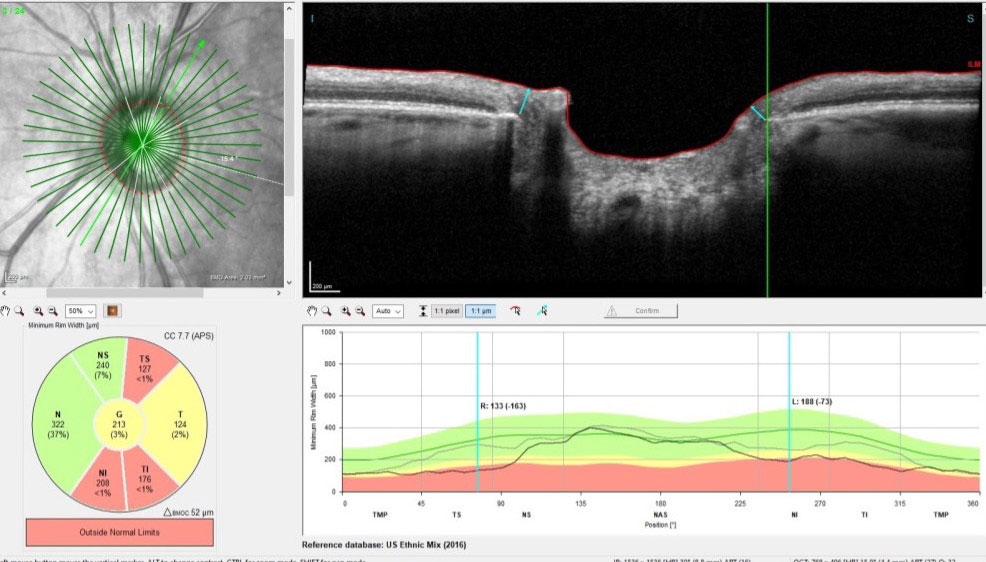
\includegraphics{../img/glaucoma/oct.jpg}

\hypertarget{introducciuxf3n}{%
\section{Introducción}\label{introducciuxf3n}}

El \href{https://es.wikipedia.org/wiki/Glaucoma}{glaucoma} es una
enfermedad ocular degenerativa que afecta al nervio óptico y es una de
las principales causas de ceguera en el mundo. El diagnóstico temprano
del glaucoma es fundamental para evitar la pérdida de visión. En este
proyecto se desarrollará un sistema de diagnóstico del glaucoma basado
en el análisis de imágenes de la retina.

\hypertarget{objetivos}{%
\section{Objetivos}\label{objetivos}}

El objetivo de este proyecto es desarrollar un sistema de diagnostico
del glaucoma basado en el análisis de imágenes de las distintas capas de
la retina obtenidas mediante una
\href{https://es.wikipedia.org/wiki/Tomograf\%C3\%ADa_de_coherencia_\%C3\%B3ptica}{tomografía
de coherencia óptica} (oct). El sistema debe ser capaz no solo de
detectar la presencia del glaucoma, sino también de cuantificar su grado
de avance, clasificando cada ojo en distintos estadios de la enfermedad.

\hypertarget{descripciuxf3n-tuxe9cnica}{%
\section{Descripción técnica}\label{descripciuxf3n-tuxe9cnica}}

La tomografía de coherencia óptica (oct) es una técnica de imagen médica
que permite obtener imágenes de alta resolución de la retina. En el caso
del glaucoma, la oct permite visualizar el nervio óptico y las distintas
capas de la retina, lo que permite detectar la presencia de daño en el
nervio óptico y cuantificar su grado de avance.

A partir de la oct se obtiene el grosor de la capa de fibras nerviosas
de la retina (RNFL) en distintos anillos de la mácula:

\begin{itemize}
\tightlist
\item
  BMO: Apertura de la membrana de Bruch por la que el nervio óptico
  abandona el globo ocular.
\item
  RIM 3.5: Anillo de 3.5 mm de diámetro centrado en el disco óptico.
\item
  RIM 4.1: Anillo de 4.1 mm de diámetro centrado en el disco óptico.
\item
  RIM 4.7: Anillo de 4.7 mm de diámetro centrado en el disco óptico.
\end{itemize}

Cada anillo se divide en 6 cuadrantes:

\begin{itemize}
\tightlist
\item
  Nasal superior
\item
  Nasal
\item
  Nasal inferior
\item
  Temporal inferior
\item
  Temporal
\item
  Temporal superior
\end{itemize}

y para cada cuadrante se mide el grosor de la capa de fibras nerviosas
de la retina en micras.

\hypertarget{tareas}{%
\section{Tareas}\label{tareas}}

\begin{enumerate}
\def\labelenumi{\arabic{enumi}.}
\tightlist
\item
  Realizar el preprocesamiento de los datos.
\item
  Realizar un análisis descriptivo de los datos de la muestra.
\item
  Investigar los distintos métodos estadísticos de clasificación
  supervisados y no supervisados y seleccionar aquellos que sean más
  adecuados para este problema de diagnóstico.
\item
  Crear un modelo de clasificación que permita detectar la presencia del
  glaucoma y cuantificar su grado de avance.
\item
  Desarrollar una aplicación que determine el estadio de glaucoma de un
  ojo a partir de los datos de una oct.
\end{enumerate}

\hypertarget{datos}{%
\section{Datos}\label{datos}}

Para el proyecto se utilizará la base de datos
\href{/datos/glaucoma.csv}{\texttt{glaucoma.csv}}. Esta base de datos
contiene las mediciones del grosor de los distintos anillos y sectores
de la capa de fibras nerviosas de la retina obtenidas mediante oct. La
base de datos incluye además el sexo, la edad y el diagnóstico de
glaucoma de cada paciente.



\end{document}
